

\subsection{Требования к времени когеренции пучка}
Время когеренции спина (spin coherence time; SCT) для метода
замороженного спина, выполненного в накопительном кольце с идеально
установленными элементами определяется минимальным детектируемым углом
отклонения вектора поляризации пучка из горизонтальной плоскости
только засчёт ЭДМ. Для уровня чувствительности $10^{-29}~e\cdot cm$
это примерно $5\cdot10^{-6}$.~\cite{BNL:Deuteron2008}

В соответствии с уравнением Т-БМТ,
\[
\W_{EDM,x} = \eta\frac{qE_x}{2mc},
\]
где $\eta$ есть коэффициент пропорциональности между ЭДМ и спином,
равный $10^{-15}$ для дейтрона, для данного уровня чувствительности.~\cite[стр.~206]{Eremey:Thesis}

Для дейтронного BNL FS кольца, $E_x = 12$
МВ/м,~\cite[стр.~19]{BNL:Deuteron2008} так что $\W_{EDM,x}\approx
10^{-9}$ рад/сек. Таким образом получаем, что для того, чтобы достичь
детектируемый уровень отклонения вектора поляризации на 1 мкрад требуется SCT порядка 1000 секунд.~\cite[стр.~207]{Eremey:Thesis}
\subsection{Происхождение декогеренции}\label{sec:decoh:origin}
Декогеренция спина в пучке вызвана разницей угловых скоростей
прецессии спинов частиц, которая, в свою очередь, вызвана разницей
длин орбит и импульсов частиц. Это можно видеть исходя из следующих
соображений.

Когда частица со спином входит в область магнитного поля, её спин-вектор
начинает поворачиваться вокруг вектора магнитного поля с угловой
скоростью определяемой уравнением Т-БМТ~\eqref{eq:TBMT_MDM}:
\begin{equation*}
	\vec\W_{MDM} = \frac qm G\vec B.
\end{equation*}
На выходе из области, вектор спина повёрнут на угол
\begin{equation*}
	\theta = \Delta t\cdot\W_{MDM} = \frac Lv \cdot \frac qm GB\cdot \frac{\gamma_0}{\gamma_0} = \frac{L\gamma_0 GB}{B\rho} = \frac L\rho\gamma_0\cdot G,
\end{equation*}
где $L$ есть длина пути внутри области с магнитным полем, и $B\rho =
p/q$ магнитная жёсткость.

В простой модели рассмотренной выше, влияние орбитальной динамики на
спиновую динамику выражено через $\gamma_0 L/\rho$ (эффективный
Лоренц-фактор). В случае референсной частицы, $\gamma_0L/\rho =
\gamma_0\alpha$, $\alpha$ угол поворота вектора импульса, в то время
как для частицы участвующей в бетатронном движении, эффективный
Лоренц-фактор больше. В следующих разделах мы выразим связь между
спиновой и орбитальной динамиками частицы в накопительном кольце в
более общих терминах.

\paragraph{Сдвиг равновесного значения импульса частицы.}
Продольная динамика заряженной частицы на референсной орбите в
накопительном кольце описывается системой уравнений
\begin{equation*}
	\begin{cases}
		\ddt{\varphi} &= -\w_{RF}\eta\delta, \\
		\ddt{\delta} &= \frac{q V_{RF}\w_{RF}}{2\pi h\beta^2E}\sin\varphi.
	\end{cases}
\end{equation*}
В уравнениях выше: $\varphi$ отклонение фазы частицы от референсной
$\varphi_0 = 0$; $\delta = \frac{\Delta p}{p_0}$ относительное
отклонение импульса от $p_0$ референсной частицы; $V_{RF}$, $\w_{RF}$
амплитуда и частоты колебаний ВЧ поля; $\eta = \alpha_0 - \gamma^{-2}$
слип-фактор, где $\alpha_0$ --- коэффициент сжатия орбиты, определяемый
через $\sfrac{\Delta L}{L} = \alpha_0\delta$, $L$ длина орбиты; $h$
гармоническое число; $E$ полная энергия ускоряемой частицы. $\w_{RF} =
2\pi h f_{rev}$, где $f_{rev}=T_{rev}^{-1}$ --- частота оборота пучка.

Решения этой системы формируют семейство эллипсов в плоскости
$(\varphi, \delta)$, центрированных на $(0,0)$. Однако, если
рассмотреть частицу, участвующую в бетатронных колебаниях, и
использовать разложение Тейлора более высокого порядка для
коэффициента сжатия орбиты $\alpha = \alpha_0 + \alpha_1\delta$,
первое уравнение системы превратится в:~\cite[стр.~2579]{Senichev:IPAC13}
\[
\ddt{\varphi} = -\w_{RF} \bkt*{\bkt{\frac{\Delta L}{L}}_\beta + \bkt{\alpha_0 + \gamma^{-2}}\delta + \bkt{\alpha_1 - \alpha_0\gamma^{-2} + \gamma^{-4}}\delta^2},
\]
где $\bkt{\frac{\Delta L}{L}}_\beta =
\frac{\pi}{2L}\bkt*{\varepsilon_xQ_x + \varepsilon_yQ_y},$ есть
удлинение орбиты, связанное с бетатронным движением; $\varepsilon_x$ и
$\varepsilon_y$ --- горизонтальный и вертикальный эмиттансы пучка, и
$Q_x$ и $Q_y$ горизонтальный и вертикальный тюны.~\cite[стр.~2580]{Senichev:IPAC13}

Решения модифицированной системы более не центрированы на одной и той
же точке. Удлинение орбиты и отклонение импульса вызывают сдвиг
равновесного значения импульса частицы~\cite[стр.~2581]{Senichev:IPAC13}
\begin{equation}\label{eq:EquLevMom_shift}
\Delta\delta_{eq} = \frac{\gamma_0^2}{\gamma_0^2\alpha_0 - 1}\bkt*{\frac{\delta_m^2}{2}\bkt{\alpha_1 - \alpha_0\gamma^{-2} + \gamma_0^{-4}} + \bkt{\frac{\Delta L}{L}}_\beta},
\end{equation}
где $\delta_m$ --- амплитуда синхротронных колебаний.

\paragraph{Понятие эффективного Лоренц-фактора.}
Равновесное значение энергии, связанное со сдвигом импульса~\eqref{eq:EquLevMom_shift}, и называемое \emph{эффективным Лоренц-фактором}, есть~\cite{Senichev:FDM}
\begin{equation}\label{eq:EffectiveGamma}
\gamma_{eff} = \gamma_0 + \beta_0^2\gamma_0\cdot\Delta\delta_{eq},
\end{equation}
где $\gamma_0$, $\beta_0$ --- Лоренц-фактор референсной частицы и
нормализованное значение
скорости. Уравнения~\eqref{eq:EquLevMom_shift}
и~\eqref{eq:EffectiveGamma} определяют связь между спиновой и
орбитальной динамиками частицы.

Из уравнения для спин-тюна частицы в магнитном поле $\nu_s = \gamma_{eff}\cdot G$ следует, что спин-тюны двух частиц с одинаковыми эффективными Лоренц-факторами равны, независимо от их траекторий в ускорителе. Этот принцип используется при использовании секступольных полей для подавления спиновой декогеренции, а также при смене полярности ведущего магнитного поля кольца.

\subsection{Подавление декогеренции с помощью секступольных полей}\label{sec:sextupole_spin_dec_solution}
Чтобы минимизировать декогеренцию спина, связанную с бетатронным
движением и отклонением импульса, могут быть использованы
секступольные (или октупольные) поля~\cite[стр.~212]{Eremey:Thesis}

Секступоль силы
\[
S_{sext} = \frac{1}{B\rho} \pddx{B_y}[x][2],
\]
где $B\rho$ магнитная жёсткость, влияет на коэффициент сжатия орбиты
первого порядка как~\cite[стр.~2581]{Senichev:IPAC13}
\begin{align}
	\Delta \alpha_{1,sext} &= -\frac{S_{sext}D_0^3}{L}, \label{eq:Sext_compaction_effect}
	\intertext{и одновременно на длину орбиты как}
	\bkt{\frac{\Delta L}{L}}_{sext} &= \mp \frac{S_{sext}D_0\beta_{x,y}\varepsilon_{x,y}}{L}, \label{eq:Sext_OL_effect}
\end{align}
где $D(s,\delta) = D_0(s) + D_1(s)\delta$ обозначает функцию дисперсии.

В следующих разделах мы будем называть декогеренцию, связанную си
горизонтальными/вертикальными бетатронными, и синхротронными
колебаниями соответственно X-/Y-, и D-декогеренцией. 

Из уравнений~\labelcref{eq:Sext_compaction_effect,eq:Sext_OL_effect} можно
видеть, что для подавления декогеренции необходимы три семейства
секступолей, помещённых в максимумы функций: $\beta_x$, $\beta_y$ для подавления
X-,Y-декогеренции, и $D_0$ для D-декогеренции.

\subsection{Симуляция секступольного подавления декогеренции в идеальном ускорителе}\label{sec:decoh:suppression_in_ideal_lattice}

Мы провели симуляцию для проверки возможности подавления декогеренции секступольными полями. В симуляции 
была использована идеальная структура с замороженным спином, описанная в разделе~\ref{chpt2:lattice:FS_BNL}.
Поскольку элементы в структуре установлены идеально, спин-векторы частиц не поворачиваются вокруг радиальной
оси; прецессия происходит только в горизонтальной слоскости, вокруг вектора $\hat y$. 

Оптимизация производится на энергии пучка 270.00 МэВ, орбитальная и спиновая трансфер-матрицы структуры
вычисляются до пятого порядка разложения ряда Тэйлора.

В структуре используются три семейства секступолей, для подавления, соответственно, декогеренции связанной 
с горизонтальными, вертикальными бетатронными колебаниями, и с синхротронными колебаниями частиц.
Оптимальное значение градиента для каждого семейства отыскивается по-отдельности; значения полей двух
других семейств зануляются. Решение оптимизировать секступоли отдельно было принято потому, что
одновременная оптимизация всех трёх градиентов вела к численным проблемам в процедуре TSS.\footnote{Также,
мы изучали принципиальную возможность оптимизации всех трёх семейств секступолей, посредством прямого
вычисления необходимых коэффициентов разложения ряда Тэйлора на трёхмерной сетке значений градиентов. 
Вопрос требует более детального рассмотрения, но на данном этапе мы сомневаемся в принципиальной возможности
оптимизации всех трёх семейств секступолей. Возможно по этой причине в~\cite[стр.~219]{Eremey:Thesis} в BNL структуре
используется всего два семейства.}

В процессе оптимизации сначала вычисляются трансфер-матрицы структуры для заданного значения градиента, 
затем процедурой TSS вычисляются разложения Тэйлора спин-тюна и оси стабильного спина. В зависимости от 
оптимизируемого семейства, из разложения спин-тюна выбирается коэффициент при квадрате соответствующей
координаты фазового пространства ($x$, $y$, или $\delta$). Модуль коэффициента служит целевой функцией: т.е., 
при оптимальном значении градиента секступолей, спин-тюн не зависит (параболически) от соответствующего отклонения частицы от референсной.

При оптимизации используется алгоритм Simplex.~\cite[стр.~37]{COSYINF:Manual:Programmer}

На Рисунке~\ref{fig:decoh:perfect} изображены зависимости спин-тюна от смещения частицы от референсной по трём
координатам фазового пространства до и после включения оптимизированных секступолей. Можно наблюдать, что во 
всех трёх случаях удалось подавить параболическую зависимость спин-тюна от коордитаны. При этом сохраняется 
линейная зависимость, которая не чувствительна к секступольным полям. Линейная зависимость наблюдается при
моделировании ускорителя в коде COSY INFINITY, в коде MODE, а также при помощи программы MAD (из личной беседы
с проф. Сеничевым). Исходя из этого, можно предположить, что эффект не является численным артефактом COSY 
INFINITY, а имеет физическое обоснование. Этот вопрос требует дальнейшего рассмотрения, но на данный момент
считается, что он подавляется соответствующей подстройкой параметров ВЧ-резонатора.~\cite[стр.~210,~219]{Eremey:Thesis}

\begin{figure}[!h]
	\centering
	\subbottom[В горизонтальном направлении]{%
		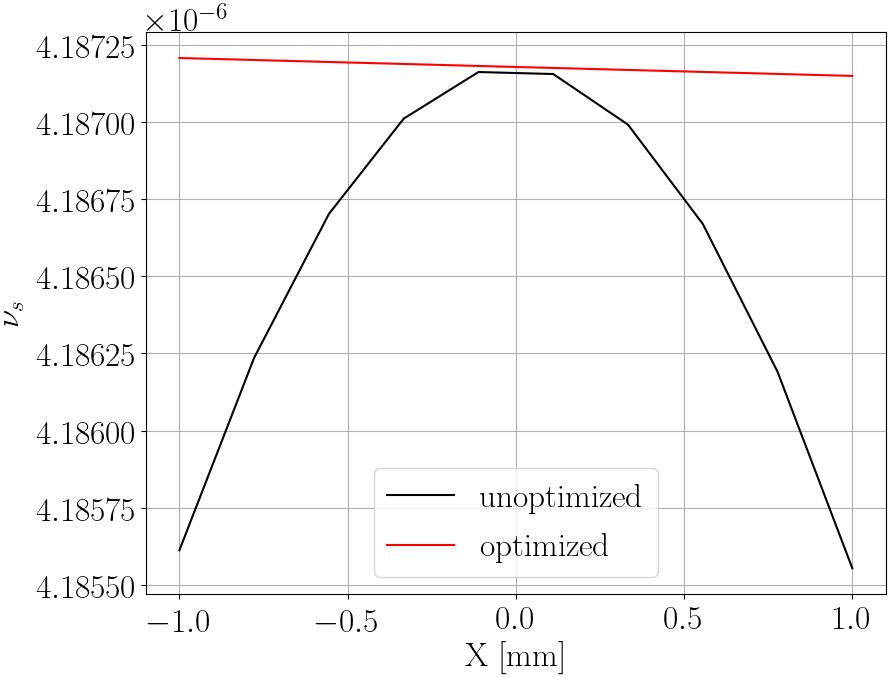
\includegraphics[height=.35\paperheight]{images/decoh_sim/spin_tune_decoh_x_offset}}
	\subbottom[В вертикальном направлении]{%
		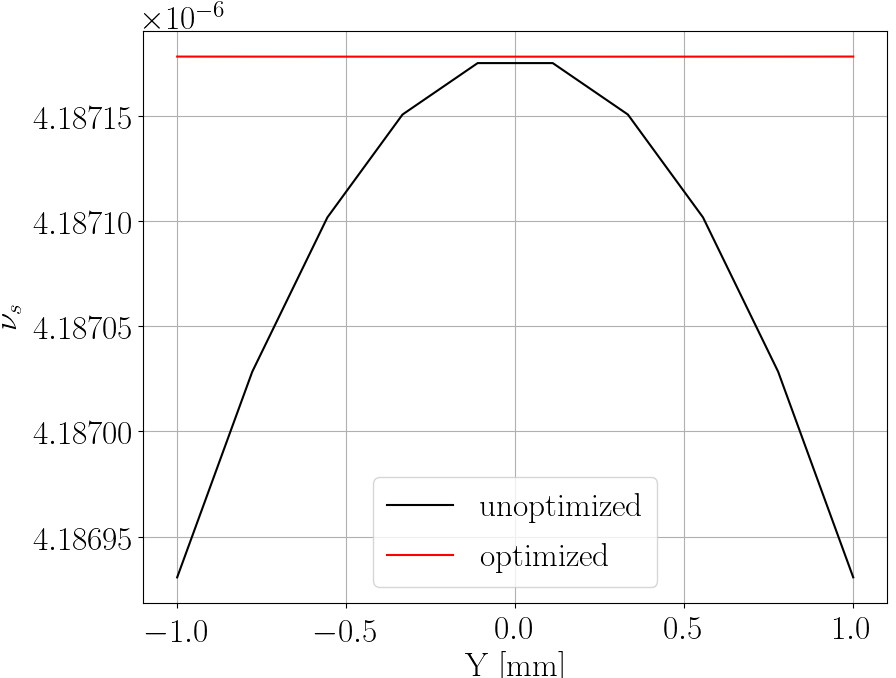
\includegraphics[height=.35\paperheight]{images/decoh_sim/spin_tune_decoh_y_offset}}
\end{figure}
\begin{figure}[!h]\centering
	\contsubbottom[По энергии]{%
		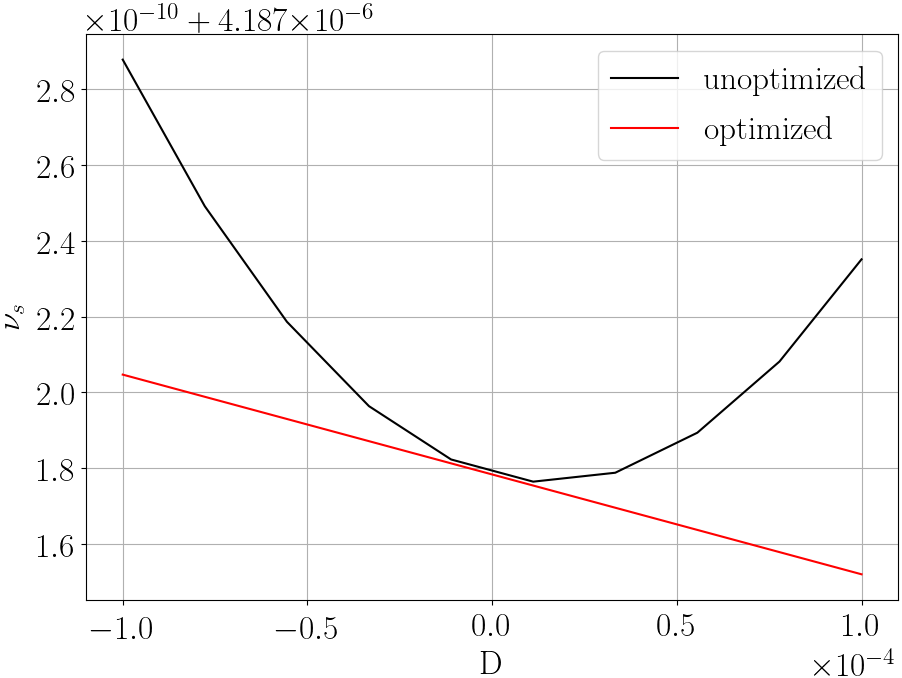
\includegraphics[height=.35\paperheight]{images/decoh_sim/spin_tune_decoh_d_offset}}
	\legend{Цветом выделены зависимости при нулевом (чёрный) и оптимизированном (красный) значениях градиента секступоля}
	\caption{Зависимость спин-тюна частицы от её смещения от референсной частицы.\label{fig:decoh:perfect}}
\end{figure}

\subsection{Переход декогеренции из горизонтальной плоскости в вертикальную, при появлении неидеальностей}
\hl{ТЕКСТ} Описывается предистория с Коопом.


В неидеальную структуру с замороженным спином инжектировался ансамбль из 30 частиц, равномерно смещённых 
от референсной в вертикальном направлении в диапазоне $y \in [-1, +1]$ мм. Поскольку анализ производится только
на основании данных трекинга, пучок инжектирован на кинетической энергии строго замороженного спина
270.0092 МэВ.

Неидеальности структуры моделируются наклонами E+B элементов вокруг оптической оси на углы, 
взятые из нормального распределения $\Theta_{tilt} \sim N(0, 1\cdot 10^{-4})$ радиан. 
Поскольку при введении таких неидеальностий сохраняется величина силы Лоренца, они не искажают 
орбитальную динамику частицы, и отражаются только на спиновой динамике. Величина стандартного отклонения
отражает реалистичную неточность установки элементов ускорителя. 

На Рисунке~\ref{fig:decoh:SX_SD} представлено стандартное отклонение радиальных компонент спин-векторов ансамбля
до и после включения секступолей. Поскольку частицы движутся в неидеальной структуре, их спин-векторы вращаются
в вертикальной плоскости с большой скоростью, и потому $\sigma_{s_x}$ --- быстро-осциллирующая функция, не
показывающая долгосрочной тенденции к росту (наклон прямой $(2\pm2)\cdot 10^{-8}$ 1/сек). Таким образом, 
не наблюдается декогеренции спина в горизонтальной плоскости. При использовании секступолей 
амплитуда колебаний $\sigma_{s_x}$ уменьшается на порядок.

На Рисунке~\ref{fig:decoh:SY_SD} представлена та же статистика  для вертикальных компонент спин-векторов. Наблюдается долгосрочный тренд, 
(наклон $(4.5 \pm 0.6)\cdot 10^{-7}$ 1/сек) до включения корректирующих секступолей. Секступольная коррекция не уменьшает амплитуду колебаний, 
но подавляет тренд (наклон после включения секступолей $(5\pm 6)\cdot 10^{-8}$ 1/сек).

\begin{figure}[h!]
	\centering
	\subbottom[Без секступолей]{%
		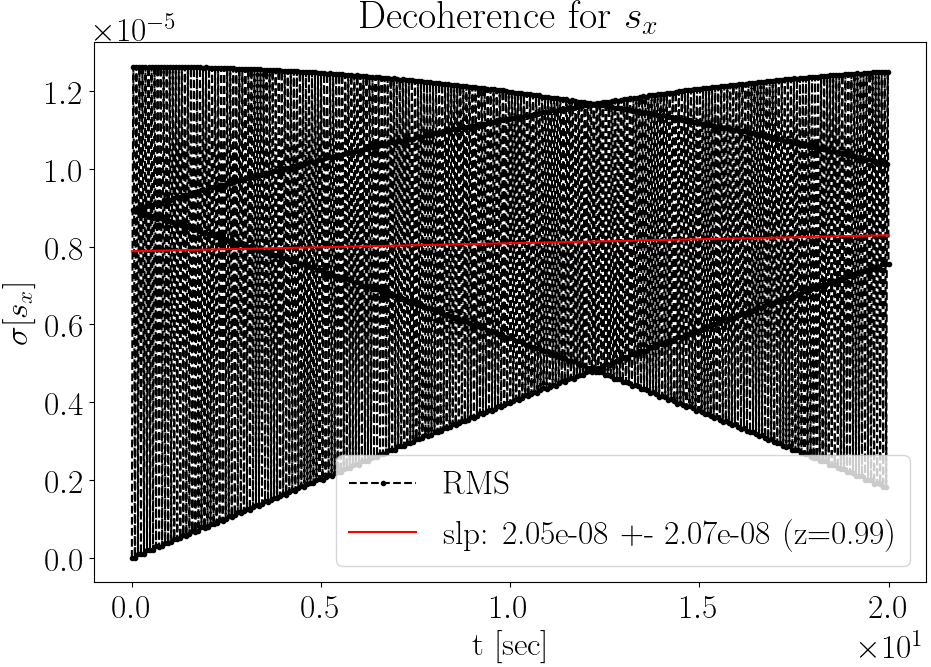
\includegraphics[height=.35\paperheight]{images/decoh_sim/SX_decoh_20sec_unopt}}
	\subbottom[С секступолями]{%
		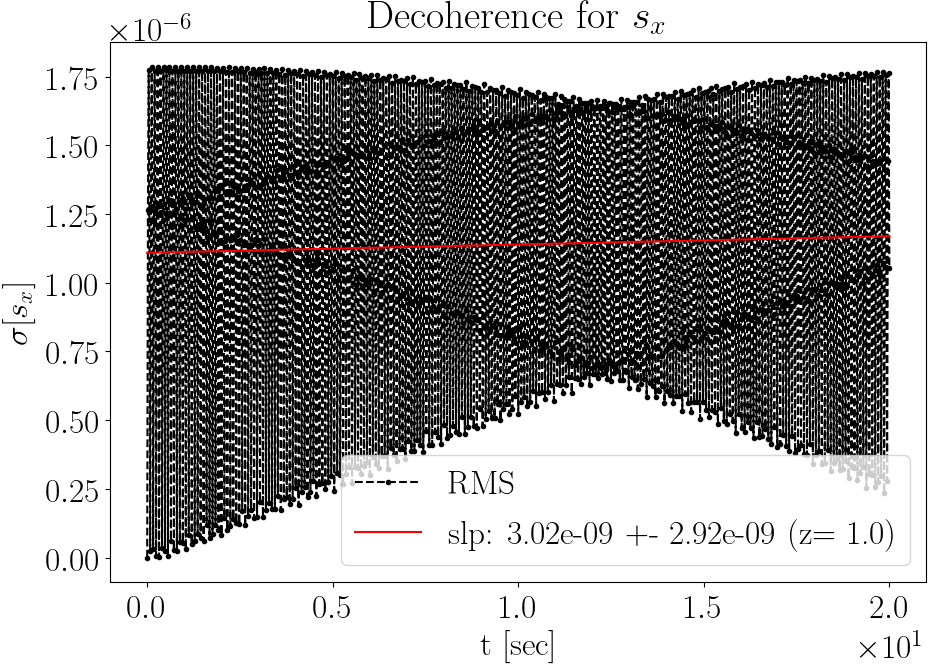
\includegraphics[height=.35\paperheight]{images/decoh_sim/SX_decoh_20sec_opt}}
	\caption{Стандартное отклонение радиальной компоненты спин-вектора частицы от спин-вектора референсной частицы\label{fig:decoh:SX_SD}}
\end{figure}

\begin{figure}[h!]
	\centering
	\subbottom[Без секступолей]{%
		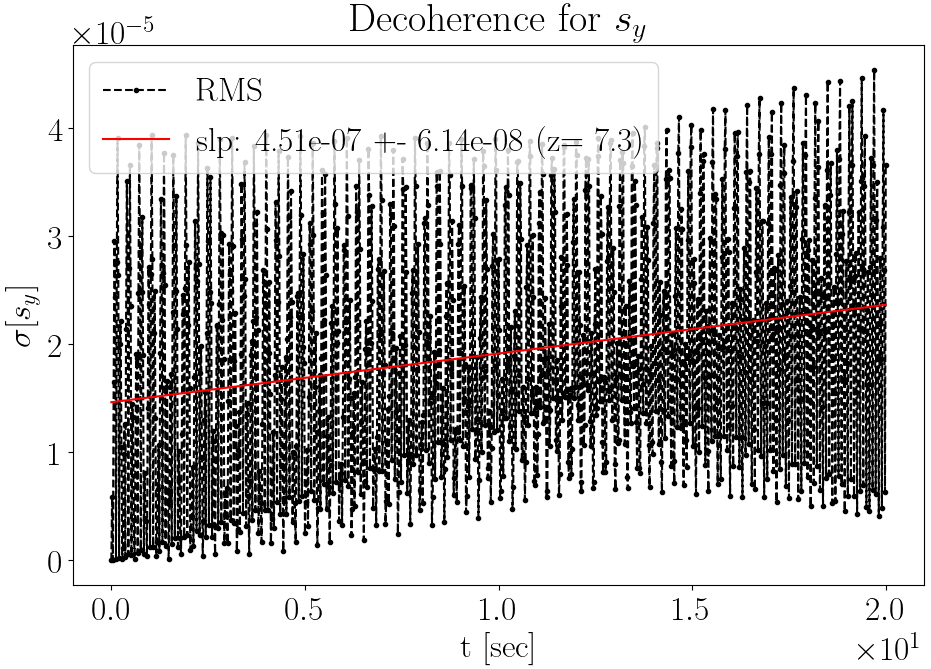
\includegraphics[height=.35\paperheight]{images/decoh_sim/SY_decoh_20sec_unopt}}
	\subbottom[С секступолями]{%
		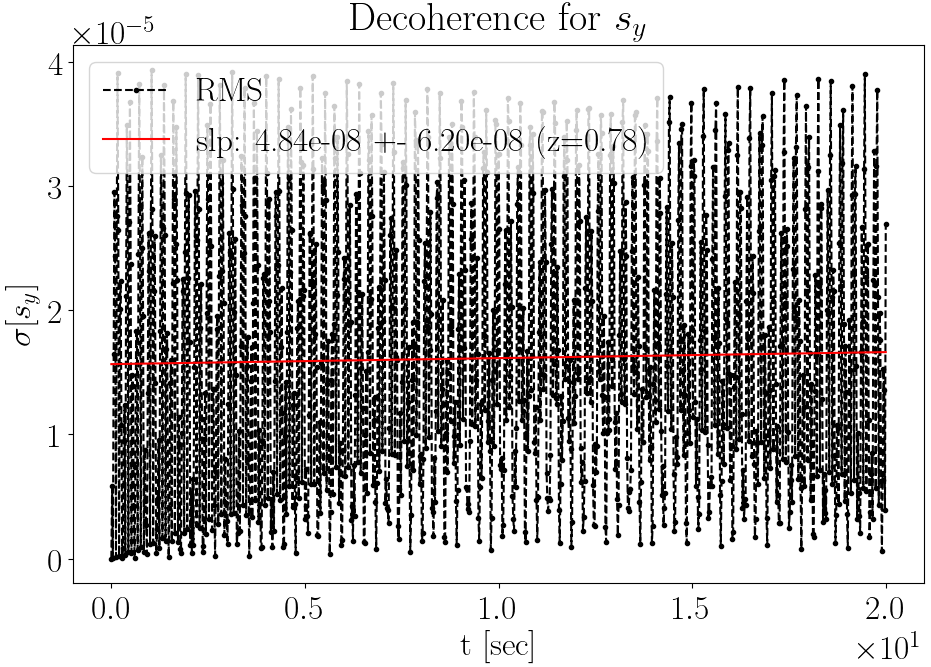
\includegraphics[height=.35\paperheight]{images/decoh_sim/SY_decoh_20sec_opt}}
	\caption{Стандартное отклонение вертикальной компоненты спин-вектора частицы от спин-вектора референсной частицы\label{fig:decoh:SY_SD}}
\end{figure}

\subsection{Симуляция эксперимента по подавлению декогеренции  неидеальном ускорителе}
При проведении нижеследующих тестов симулировалась инжекция
плоского, гауссовского пучка в структуру с замороженным
спином. E+B спин-ротаторы в структуре были установлены со случайно распределённым углом наклона вокруг оптической оси, взятым из распределения $N(0, 5\cdot10^{-4})$ радиан.

Инжектируемые пучки состояли из 30 частиц, распределённых в вертикальной
плоскости $y-z$ как $y\sim N(y_0, 0.1)$ мм; все остальные координаты равны нулю.
Оффсет $y_0$ варьировался в диапазоне $[-1, +1]$ мм. Начальное
направление спин-векторов всех частиц --- продольное: $\vec S(t=0) = (0,0,1)$.

Также в структуре варьировалось значение градиента $G_Y$ секступоля,
модулирующего декогеренцию в вертикальной плоскости. $G_Y$ менялся в
диапазоне $[G_Y^0 - 5\cdot10^{-3}, G_Y^0 + 5\cdot10^{-3}]$, где
$G_Y^0=-5.77\cdot 10^{-4}$ --- оптимальное значение градиента для заданных 
неидеальностей структуры. Величина $G_Y^0$ была найдена путём минимизации коэффициента разложения $a_2$
ряда Тэйлора $\nu_s(y) \approx a_0 + a_1\cdot y + a_2\cdot y^2 + O(y^3)$.

На каждое значение градиента приходится 10 инжекций.

Для того, чтобы обеспечить устойчивость процедуры TSS COSY Infinity~\cite{COSYINF:BeamPhysMan}, пучок инжектировался на энергии 270 МэВ (строгий FS находится на энергии 270.0092 МэВ), а матрицы перехода орбитального и спинового движений строились до третьего порядка разложения ряда Тейлора. 

Далее ансамбль начальных значений, представляющий пучок, трекается
через структуру на протяжении $1.2\cdot10^6$ оборотов, что
примерно эквивалентно 1.2 секундам. Каждые 800 оборотов производится
запись необходимых для анализа данных.

Собираемые данные: 
\begin{enumerate*}[\itshape a\upshape)]
	\item результаты вычислений процедуры TSS: спин-тюн $\nu_s$ и компоненты вектора оси инвариантного спина $\bar n$, и
	\item компоненты спина $(S_X, S_Y, S_Z)$, и фазового пространства $(X,A,Y,B,T,D)$.
\end{enumerate*}
Мы также записывали разложения ряда Тэйлора функций $\nu_s$, $\nbar$, орбитальной, и спиновой трансфер матриц
структур для каждого значения $G_Y$.

Из данных по компонентам спина вычисляется вектор поляризации банча:
\begin{equation}\label{eq:polarization_formula}
\vec P = \frac{\sum_i\vec s_i}{|\sum_i\vec s_i|}.
\end{equation}

Вертикальная компонента вектора фиритуется функцией $f(t; a,f,\phi) = a\cdot \sin(2\pi\cdot
f\cdot t + \phi)$, оцениваются все три параметра $(\hat a, \hat f,
\hat\phi)$. 

\subsection{Анализ эффекта подавления декогеренции спина в вертикальной плоскости при помощи секступолей}
На Рисунке~\ref{decoh:fig:ny_vs_y0_GSY} представлена зависимость вертикальной компоненты оси стабильного спина частицы от её вертикального смещения от референсной орбиты: $\nbar_y(y)\approx a_0 + a_1\cdot y + a_2\cdot y^2 + O(y^3)$. На Рисунке~\ref{decoh:fig:full:ny_vs_y0_GSY} можно наблюдать разгибание ветвей параболы при $G_Y \rightarrow G_Y^0$. Присутствие в разложении $\nbar_y(y)$ линейного члена обнаруживается на 
Рисунке~\ref{decoh:fig:zoom:ny_vs_y0_GSY}.

\begin{figure}[h!]
	\centering
	\subbottom[Полный диапазон.\label{decoh:fig:full:ny_vs_y0_GSY}]{%
		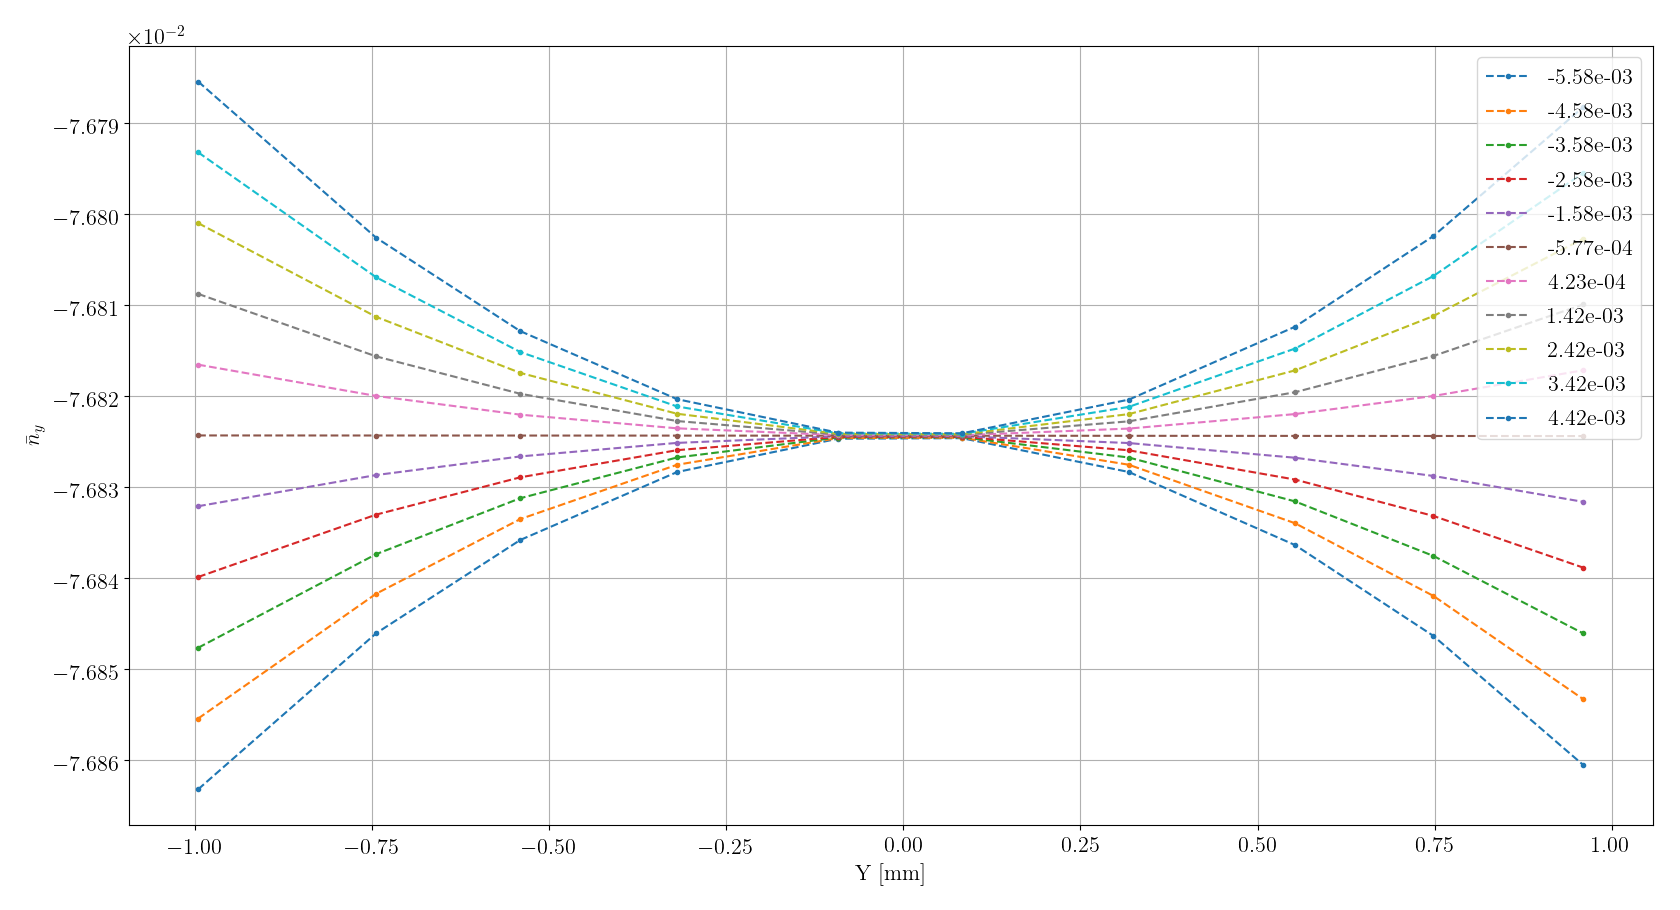
\includegraphics[width=\linewidth]{images/decoh_sim/ny_vs_offset}}
	\subbottom[Деталировка кривой при оптимальном значении $G_Y$.\label{decoh:fig:zoom:ny_vs_y0_GSY}]{%
		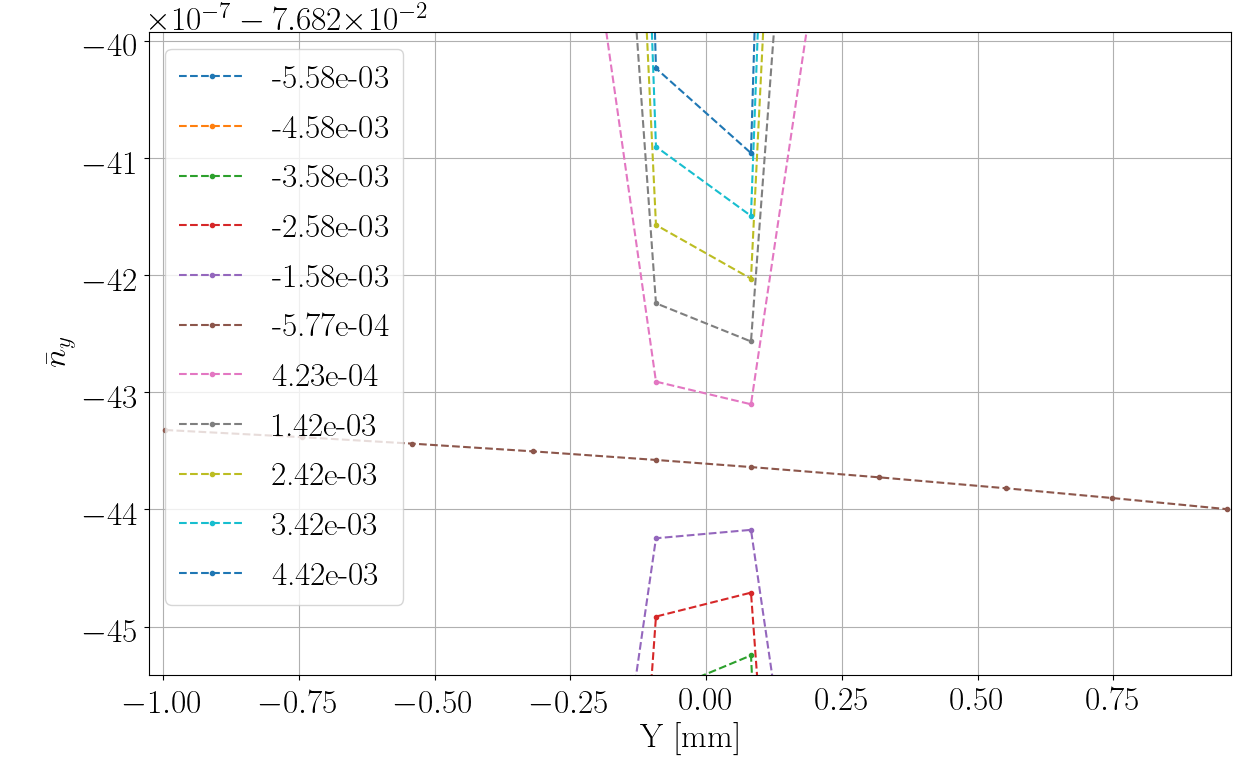
\includegraphics[width=\linewidth]{images/decoh_sim/ny_vs_offset_zoom}}
	\legend{Цветом обозначены данные для различных значений градиента $G_Y$ Y-секступоля.}
	\caption{Вертикальная компонента $\bar n_y$ оси прецессии спина в зависимости от смещения частицы от референсной орбиты.\label{decoh:fig:ny_vs_y0_GSY}}
\end{figure}

На Рисунке~\ref{decoh:fig:ST_vs_y0_GSY} представлена зависимость спин-тюна от вертикального смещения частицы от референсной орбиты.
\begin{figure}[h!]
	\centering
	\subbottom[Полный диапазон~\label{decoh:fig:full:ST_vs_y0_GSY}]{%
		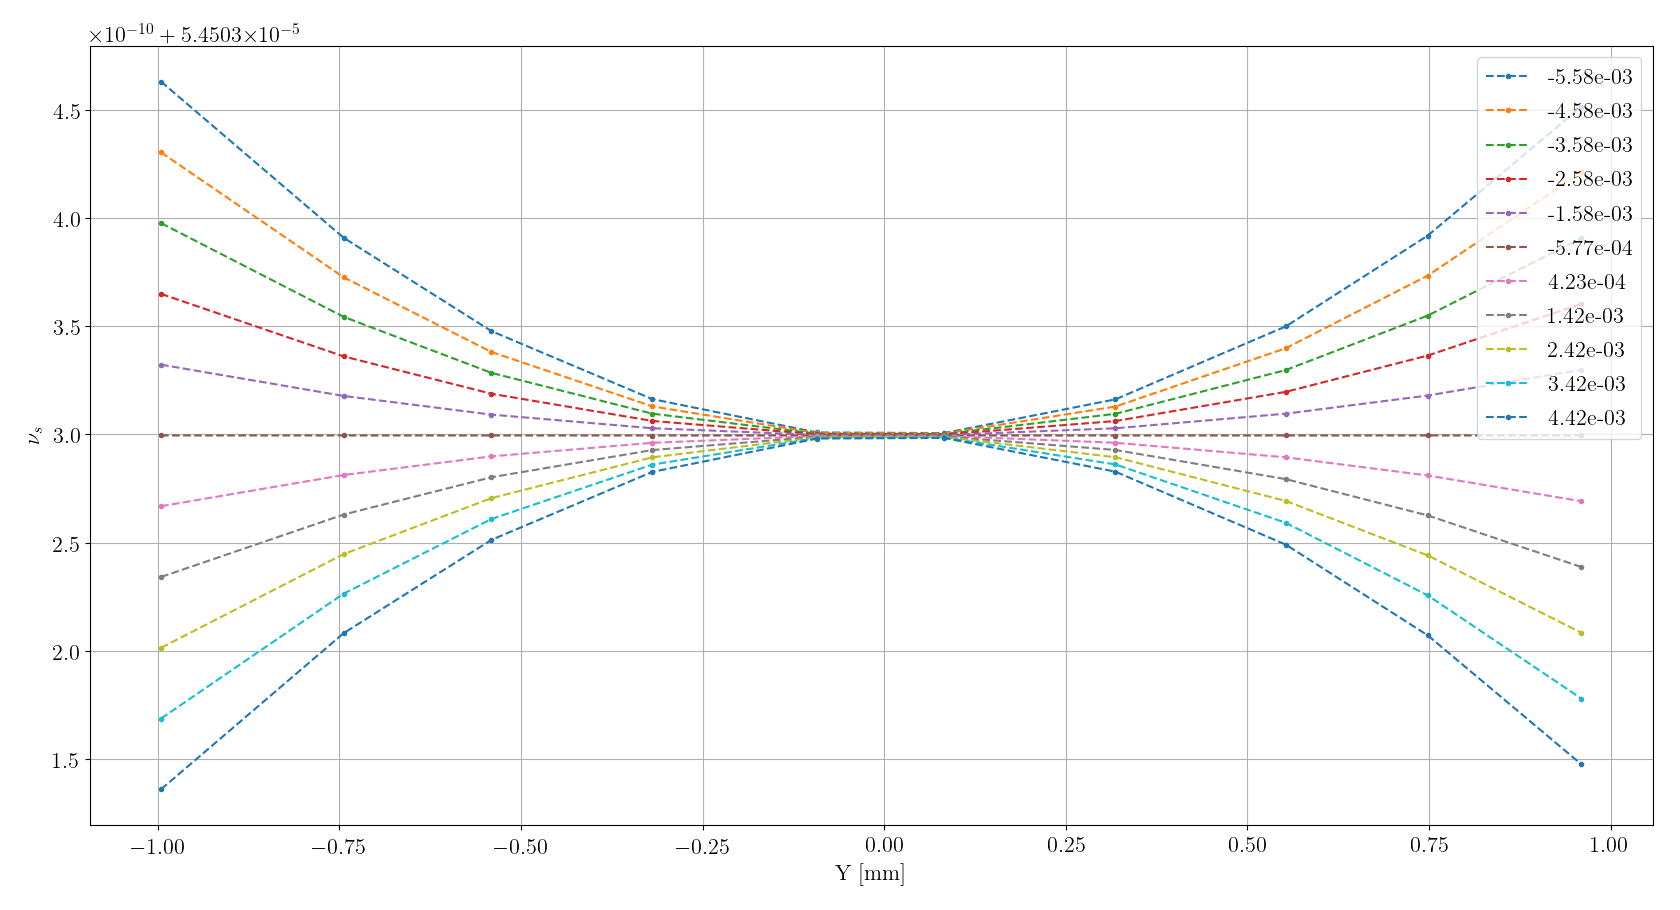
\includegraphics[width=\linewidth]{images/decoh_sim/spin_tune_vs_offset}}
	\subbottom[Деталировка кривой при оптимальном значении $G_Y$\label{decoh:fig:zoom:ST_vs_y0_GSY}]{%
		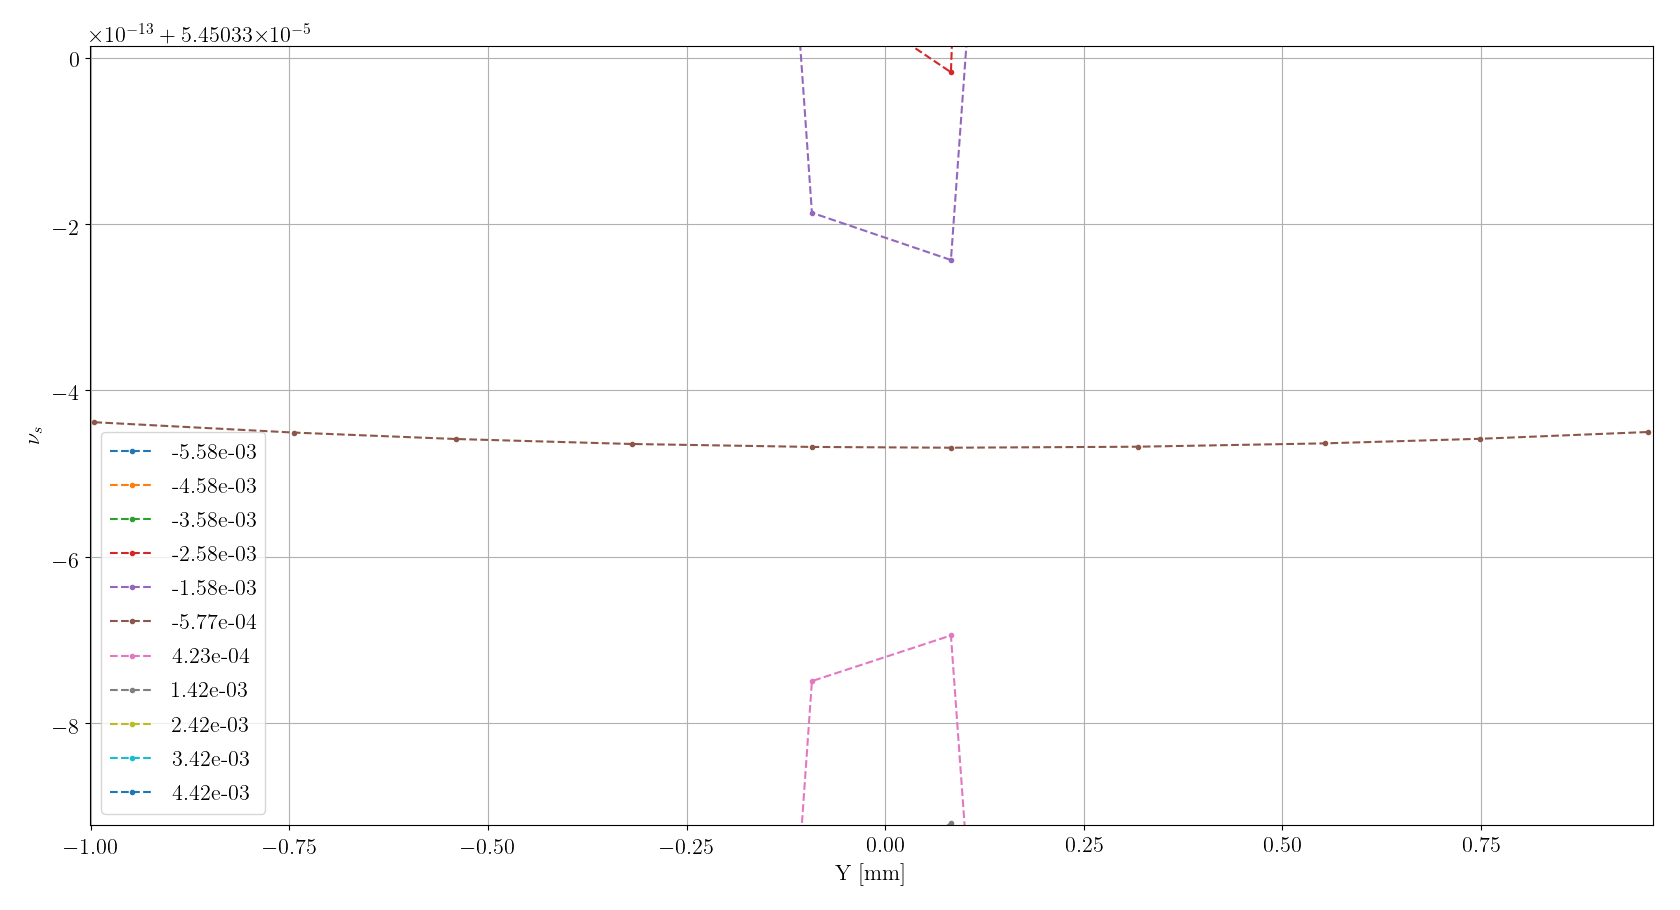
\includegraphics[width=\linewidth]{images/decoh_sim/spin_tune_vs_offset_zoom}
	}
	\legend{Цветом обозначены данные для различных значений градиента $G_Y$ Y-секступоля.}
	\caption{Спин-тюн $\nu_s$ в зависимости от смещения частицы от референсной орбиты.\label{decoh:fig:ST_vs_y0_GSY}}
\end{figure}

На Рисунке~\ref{decoh:fig:yb_traj} изображены траектории частиц в плоскости $(Y,B)$ фазового пространства, полученные в результате трекинга через неидеальный ускоритель.
\begin{figure}[h!]
	\centering
	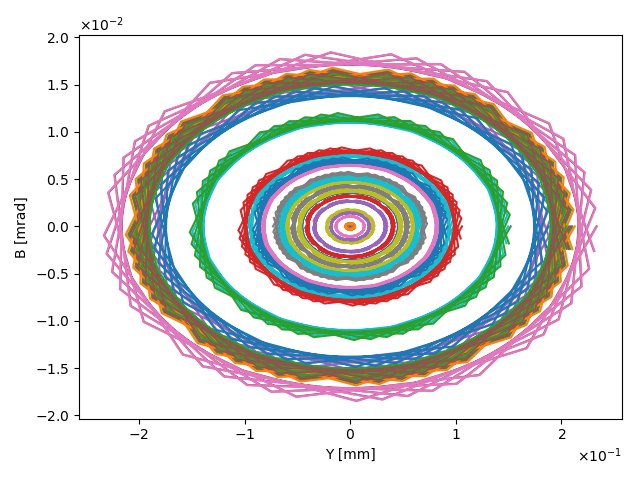
\includegraphics[width=\linewidth]{images/decoh_sim/YB-PHASE_SPACE_IMPERFECT_UNOPT}
	\caption{Траектории частиц в плоскости $(Y,B)$ фазового пространства.\label{decoh:fig:yb_traj}} 
\end{figure}

На Рисунках~\ref{decoh:fig:ST_on_traj}, \ref{decoh:fig:NX_on_traj}, \ref{decoh:fig:NY_on_traj}, и \ref{decoh:fig:NZ_on_traj} изображены, соответственно: спин-тюн, радиальная, вертикальная, и продольная компоненты оси прецессии спина, вычисленные на траекториях частиц из Рисунка~\ref{decoh:fig:yb_traj}, в двух случаях:
\begin{enumerate*}[\itshape i\upshape)]
	\item с выключенными, и 
	\item с включенными секступолями $G_Y$.
\end{enumerate*}  

\begin{figure}[!h]
	\centering
	\subbottom[С выключенными секступолями.]{%
		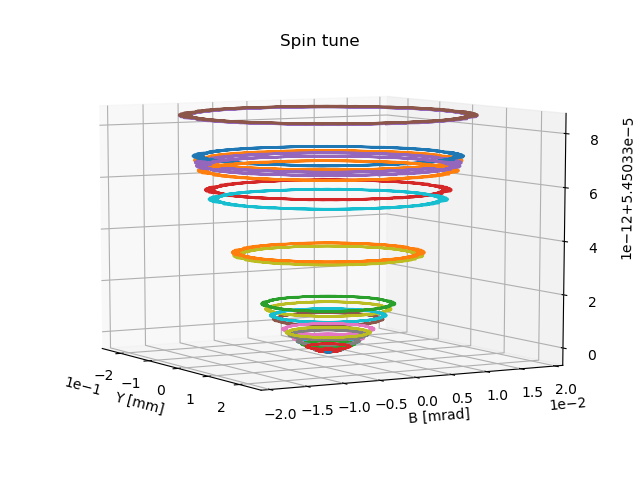
\includegraphics[width=\linewidth]{images/decoh_sim/ST_VS_YB_IMPERFECT_UNOPT}}
	\hfill
	\subbottom[С включенными секступолями.]{%
		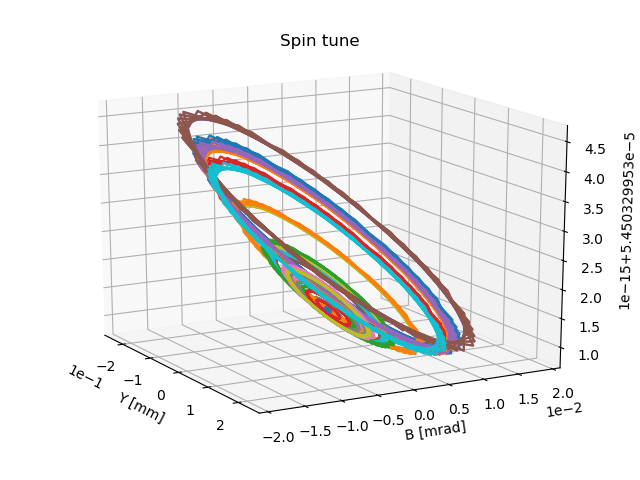
\includegraphics[width=\linewidth]{images/decoh_sim/ST_VS_YB_IMPERFECT_OPTIM}}
	\hfill
	\caption{Спин-тюны частиц на их траекториях в неидеальной FS-труктуре.\label{decoh:fig:ST_on_traj}}
\end{figure}

\begin{figure}[!h]
	\centering
	\subbottom[С выключенными секступолями.]{%
		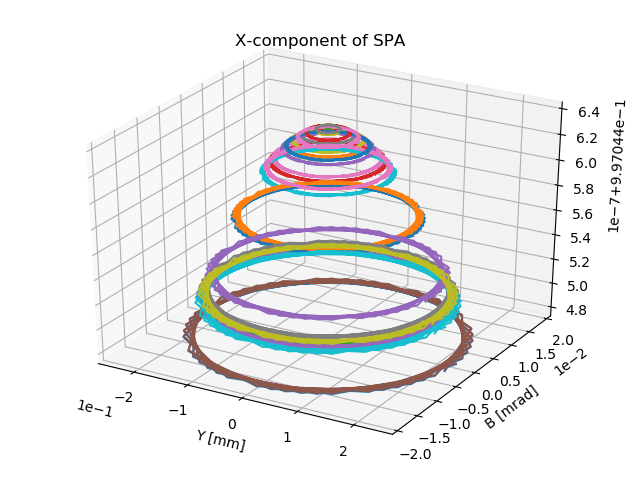
\includegraphics[width=\linewidth]{images/decoh_sim/NX_VS_YB_IMPERFECT_UNOPT}}
	\hfill
	\subbottom[С включенными секступолями.]{%
		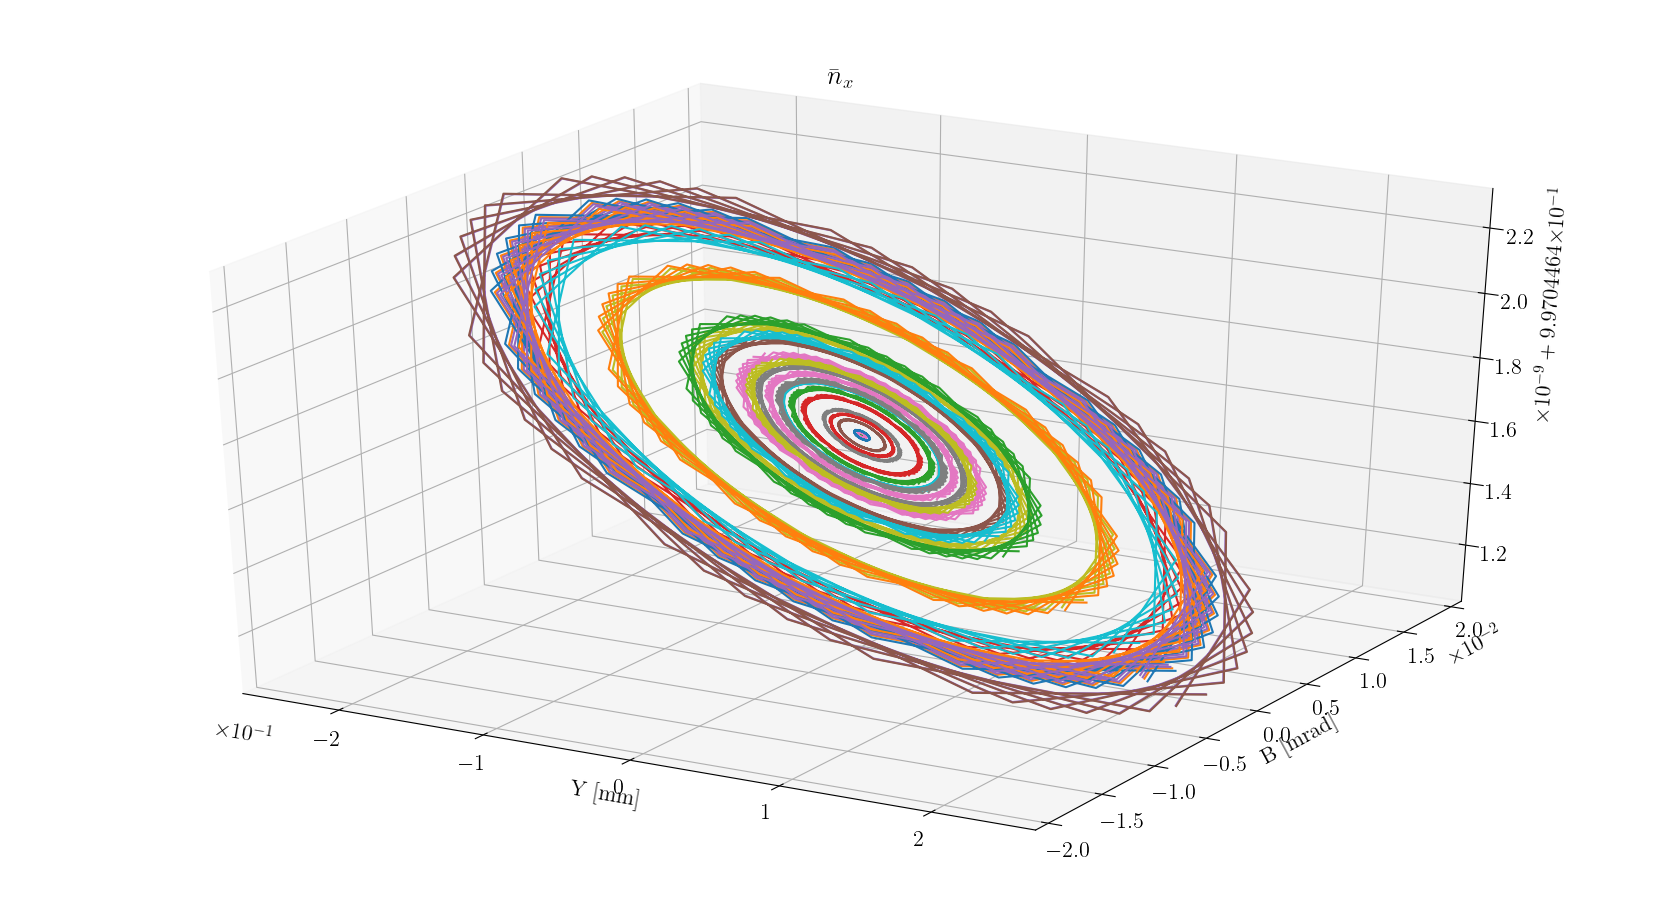
\includegraphics[width=\linewidth]{images/decoh_sim/NX_VS_YB_IMPERFECT_OPTIM}}
	\hfill
	\caption{Радиальные компоненты осей прецессии спинов частиц на их траекториях в неидеальной FS-труктуре.\label{decoh:fig:NX_on_traj}}
\end{figure}

\begin{figure}[!h]
	\centering
	\subbottom[С выключенными секступолями.]{%
		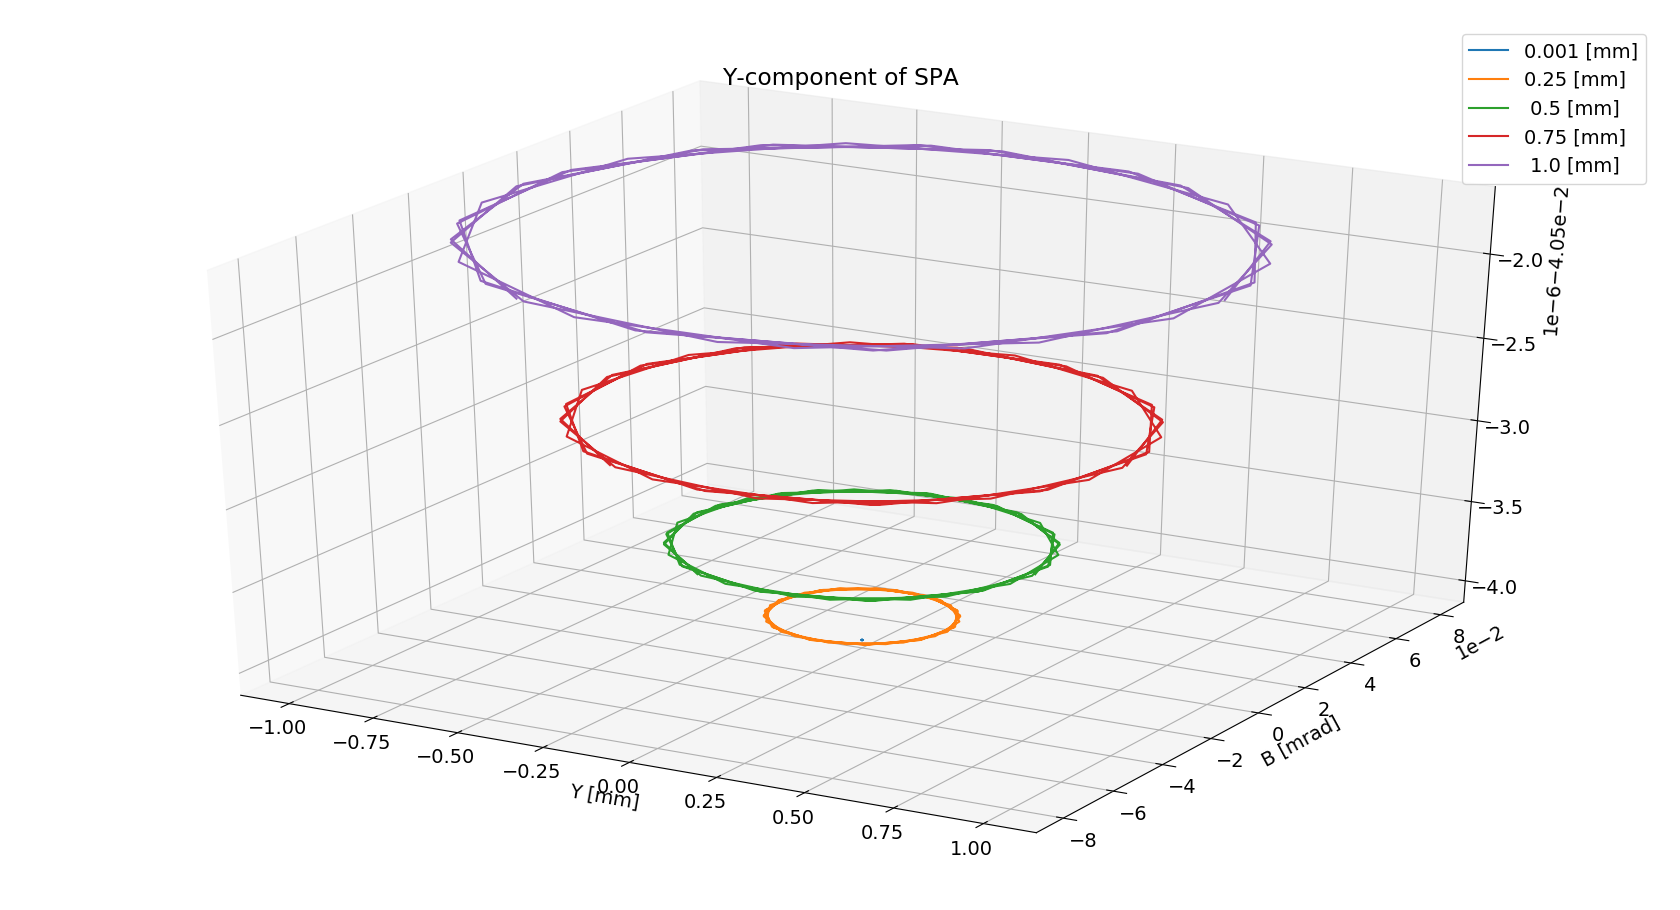
\includegraphics[width=\linewidth]{images/decoh_sim/NY_VS_YB_IMPERFECT_UNOPT}}
	\hfill
	\subbottom[С включенными секступолями.]{%
		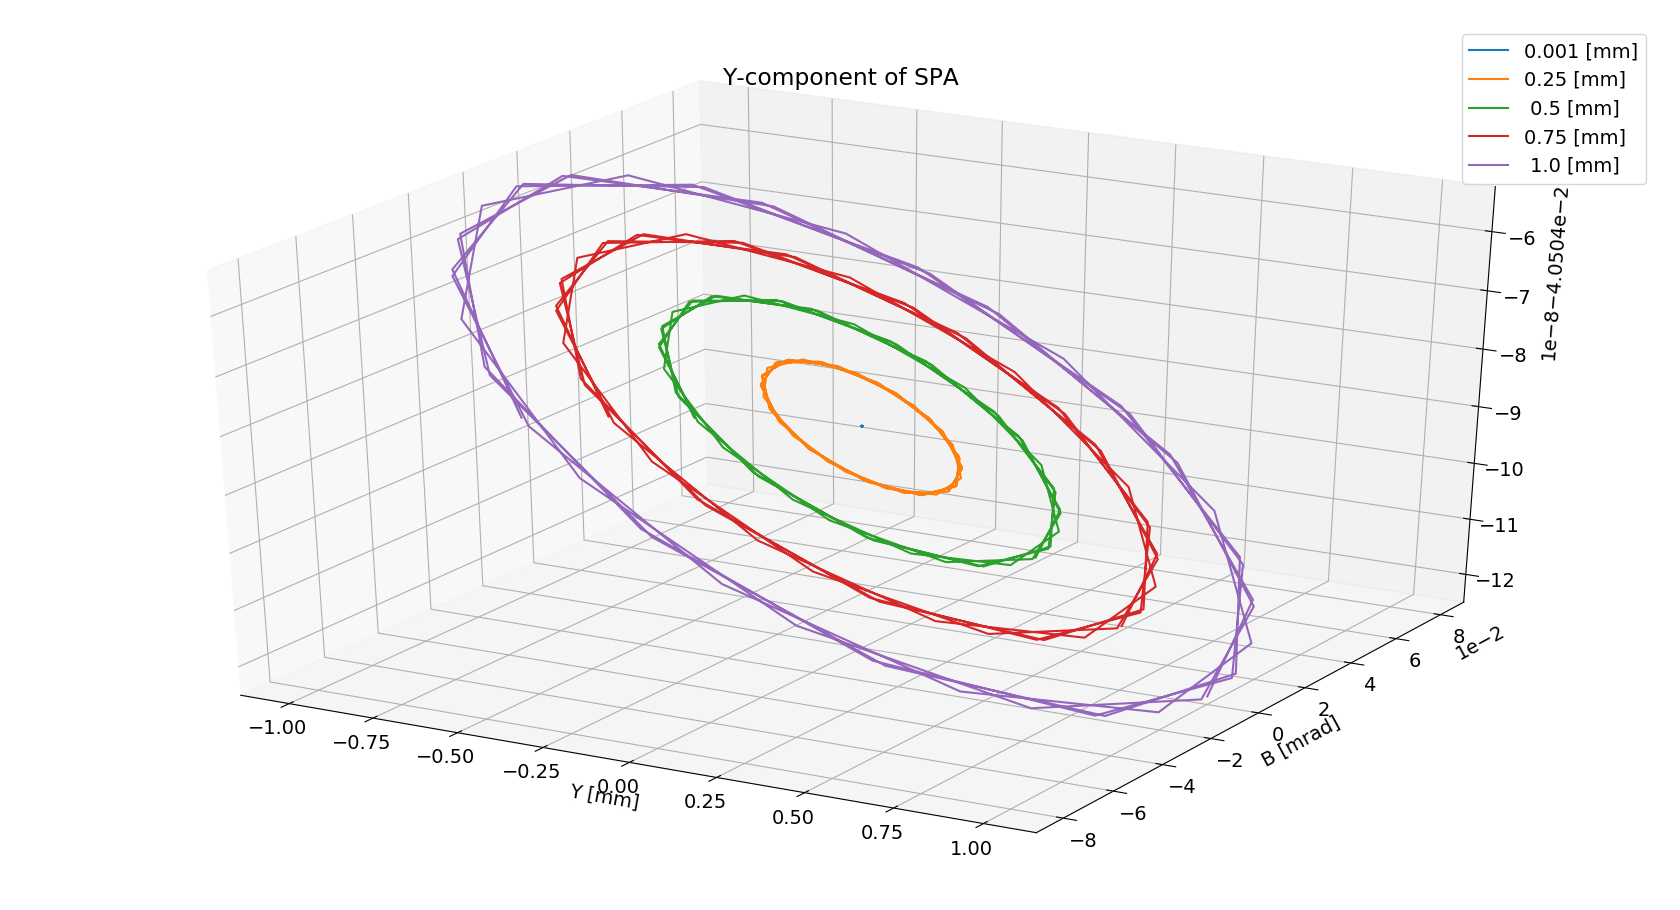
\includegraphics[width=\linewidth]{images/decoh_sim/NY_VS_YB_IMPERFECT_OPTIM}}
	\hfill
	\caption{Вертикальные компоненты осей прецессии спинов частиц на их траекториях в неидеальной FS-труктуре.\label{decoh:fig:NY_on_traj}}
\end{figure}

\begin{figure}[!h]
	\centering
	\subbottom[С выключенными секступолями.]{%
		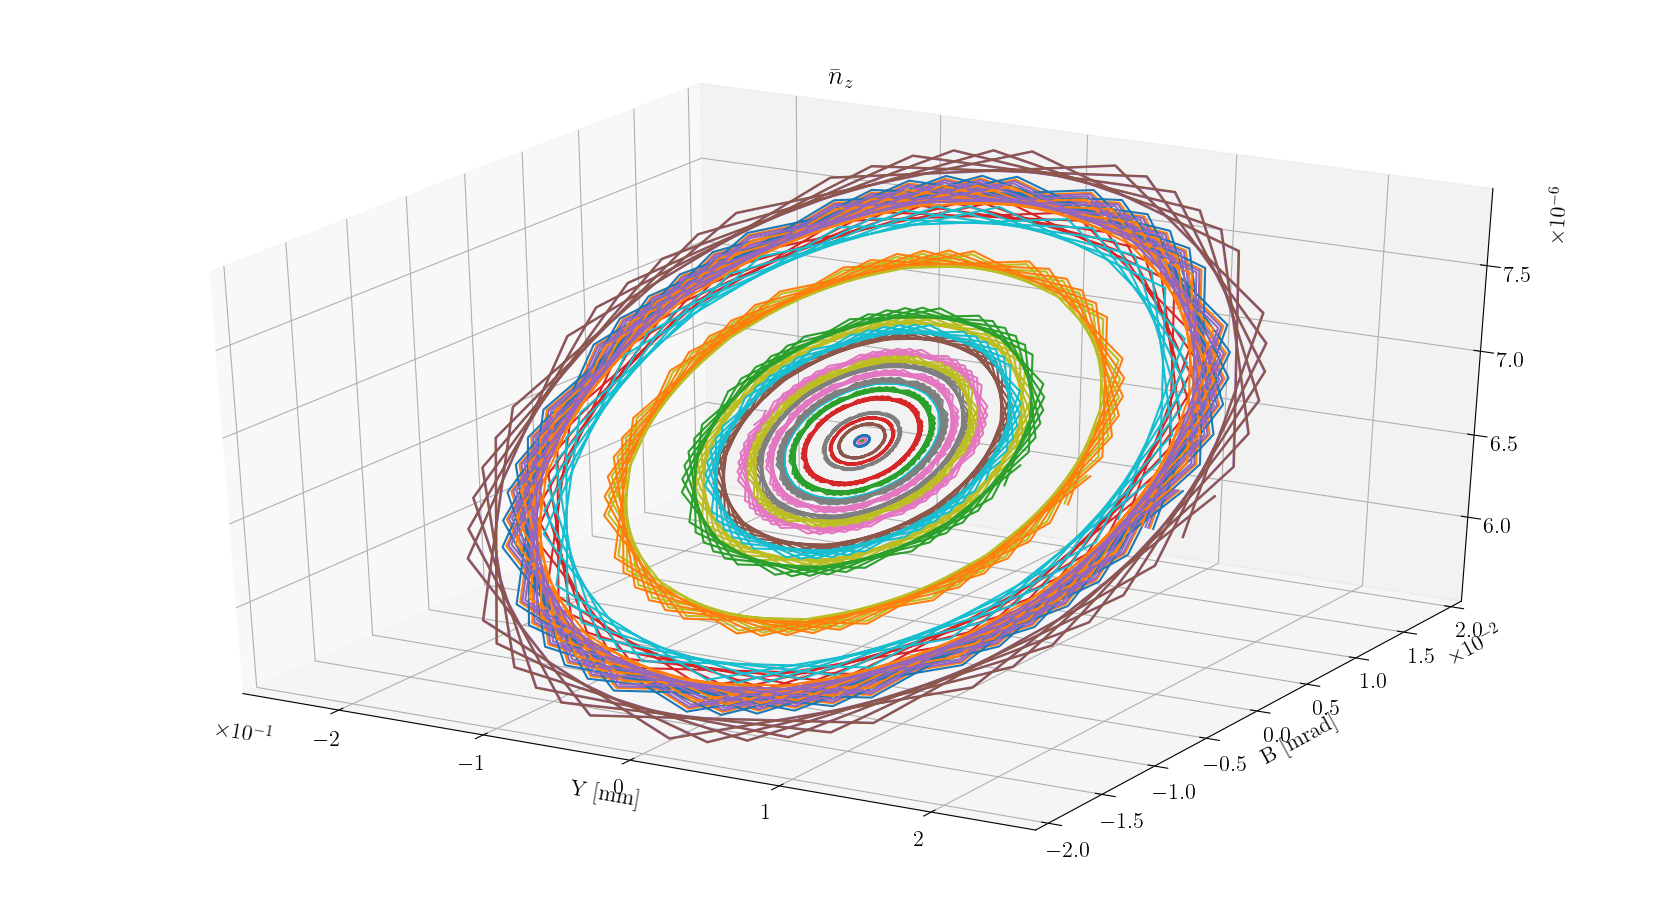
\includegraphics[width=\linewidth]{images/decoh_sim/NZ_VS_YB_IMPERFECT_UNOPT}}
	\hfill
	\subbottom[С включенными секступолями.]{%
		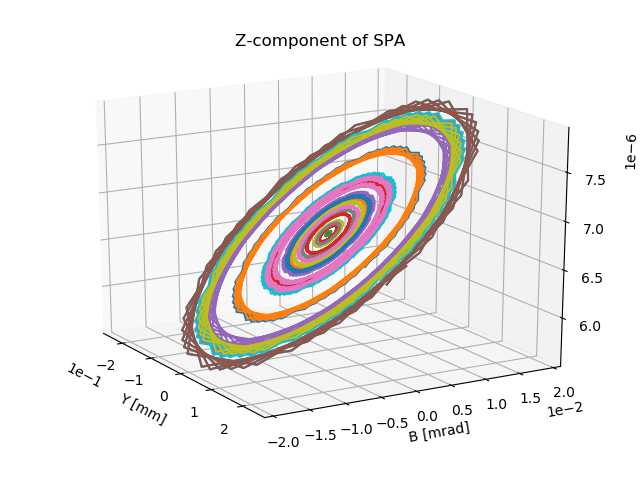
\includegraphics[width=\linewidth]{images/decoh_sim/NZ_VS_YB_IMPERFECT_OPTIM}}
	\hfill
	\caption{Продольные компоненты осей прецессии спинов частиц на их траекториях в неидеальной FS-труктуре.\label{decoh:fig:NZ_on_traj}}
\end{figure}

Исходя из рисунков можно отметить следующее:
\begin{enumerate}
	\item в безсекступольном случае, и $\nu_s$ и направление $\nbar$ частицы по большей части (с точностью до влияния линейного члена разложения) фиксированы величиной её поперечного эмиттанса;
	\item при применении секступольных полей, уровни $\nu_s$ и $\nbar$ сравниваются, и становится виден эффект бетатронных колебаний, связанный с присутствием в разложении Тэйлора функций линейной компоненты.
\end{enumerate}
Таким образом, Рисунки~\ref{decoh:fig:NX_on_traj} и~\ref{decoh:fig:NY_on_traj} свидетельствуют о том, что применение секступольных полей не только выравнивает модули частот прецессии частиц банча, но и их направления. Продольная компонента оси стабильного спина не чувствительна к секступольным полям, как видно из Рисунка~\ref{decoh:fig:NZ_on_traj}.


На Рисунке~\ref{decoh:fig:nbar_vs_ST} представлены зависимости средних значений (уровней) радиальной и вертикальной компонент оси стабильного спина частицы от среднего значения её спин-тюна. 
\begin{figure}[!h]
	\centering
	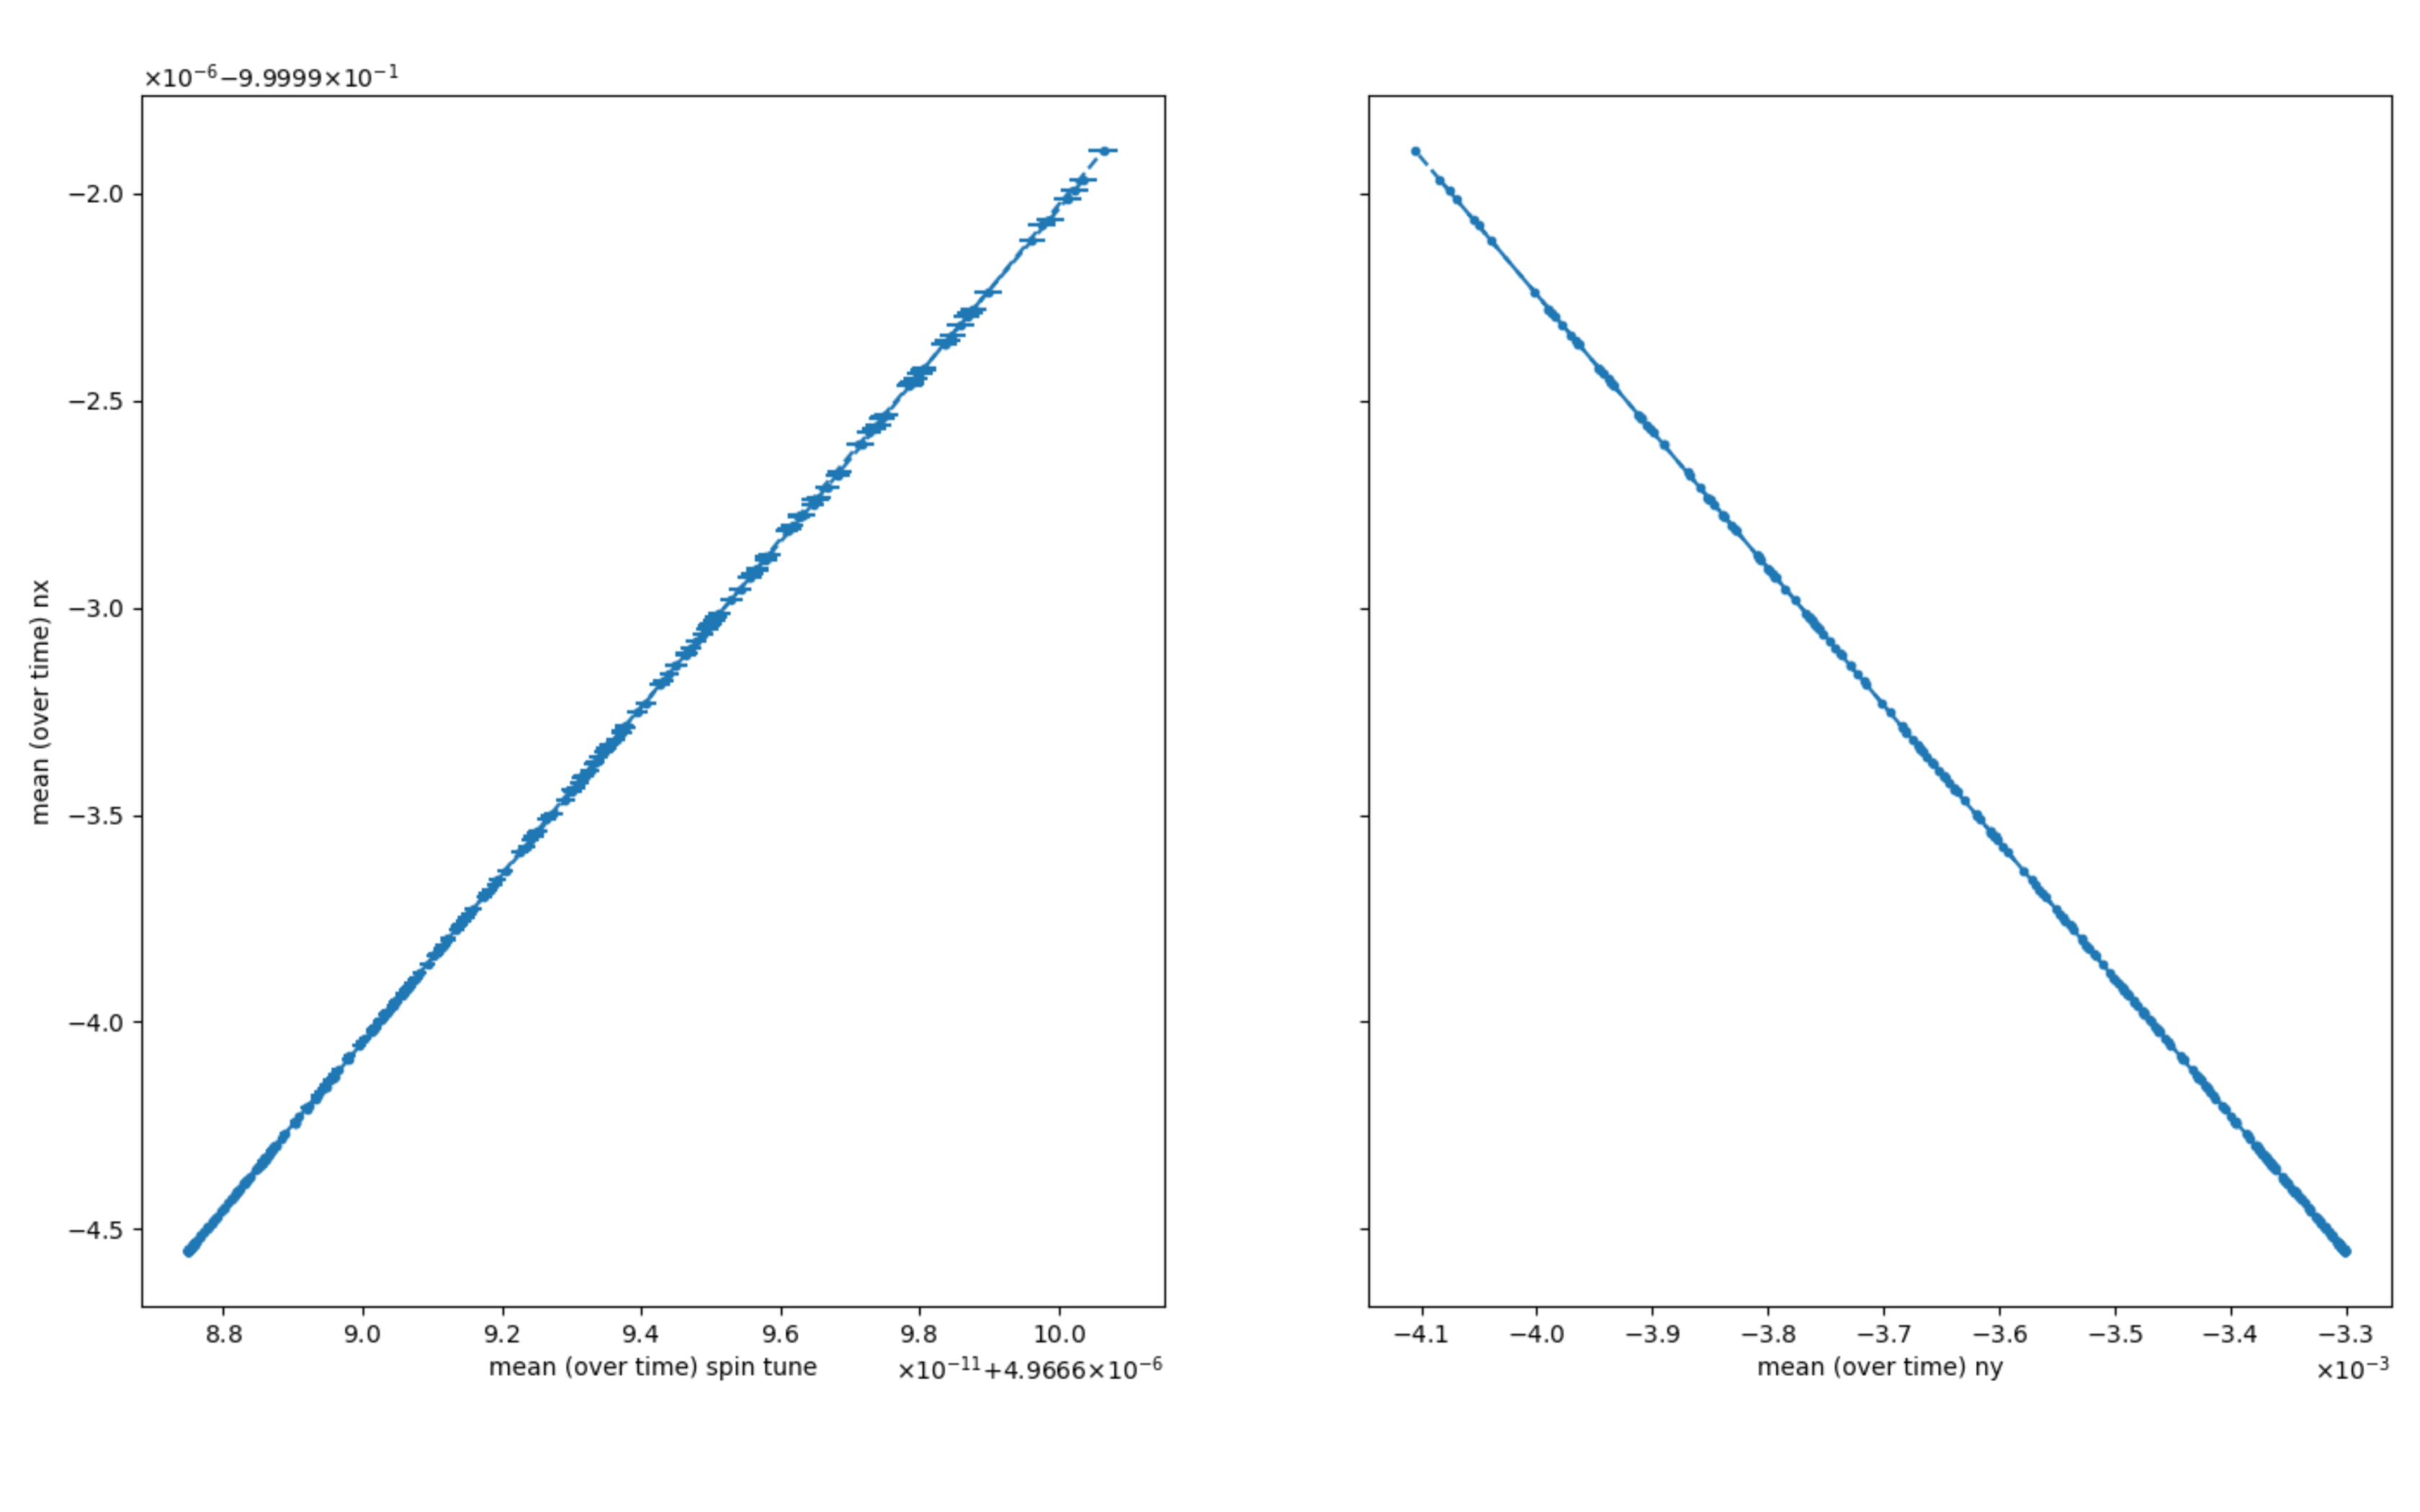
\includegraphics[width=\linewidth]{images/decoh_sim/mean_n_bar_vs_spin_tune}
	\caption{Средние уровни поперечных компонент осей стабильного спина частиц, в зависимости от уровня их спин-тюна.\label{decoh:fig:nbar_vs_ST}}
\end{figure}

